%%%%%%%%%%%%%%%%%%%%%%%%%%%%%%%%%%%%%%%%%%%%%%%%%%%%%%%%%%%%%%%%%%%%%%%%
%                                                                      %
%     File: Thesis_Introduction.tex                                    %
%     Tex Master: Thesis.tex                                           %
%                                                                      %
%     Author: Andre C. Marta                                           %
%     Last modified :  2 Jul 2015                                      %
%                                                                      %
%%%%%%%%%%%%%%%%%%%%%%%%%%%%%%%%%%%%%%%%%%%%%%%%%%%%%%%%%%%%%%%%%%%%%%%%

\chapter{Introduction}
\label{chapter:introduction}

The number of reported security breaches due to \emph{virus}, \emph{trojans}, \emph{ransomwares}, etc, has been growing considerably in recent years~\cite{av-test:report} with reports of infections due to \emph{malware}  making the headlines, now more than ever.
Almost every week one such security vulnerability is reported which may be seen as a failure by the security community on the control and detection of malicious content. 

Due to the significant number of malware attacks, and taking into consideration the increasing popularity and huge success of \gls{ml} methodologies in classification in different domains~\cite{lee2003learning,joachims2002learning,li2010object,ding2001multi}, it is only natural to see these techniques applied to complement classical methodologies for malicious-content detection~\cite{arp2014drebin,christodorescu:semantics,kolosnjaji2016deep,kolter:learning,miller:rev_int,nissim:al_pdf,perdisci:behavior,rieck:dynamic,santos2013opcode,schultz:data_mining,schwenk2012autonomous,vsrndic2013detection,deo2016prescience,gandotra2014malware,jordaney2017transcend,rossow:practices}, in particular, supervised learning techniques.

%%%%%%%%%%%%%%%%%%%%%%%%%%%%%%%%%%%%%%%%%%%%%%%%%%%%%%%%%%%%%%%%%%%%%%%%
\section{Motivation}
\label{section:motivation}

Malware, which can be referred to by other names like malicious software or malicious code, can be described as \say{any code added, changed, or removed from a software system in order to	intentionally cause harm or subvert the intended function of the system}~\cite{mcgraw:mal_code}.
Malware can be a piece of code attached to a legitimate program, an independent program, or a combination of both.

The reasoning that leads to malware creation varies greatly, some are created to demonstrate some vulnerability or concept and do not cause direct harm to systems, while others are used to steal information or render systems useless.
The wide variety and quantity of now-a-day systems and the amount of sensitive information they store provide numerous opportunities to illegally make a profit out of subverting legitimate systems.

The amount of malware has shown an exponential increase since the early 2000s, from 1 million in 2006 to over 500 million by the end of 2016~\cite{av-test:report,mcafee:report}. According to a 2007 study by McAfee\footnote{McAfee Study Finds 4 Percent of Search Results Malicious, by Frederick Lane, June 4, 2007 [http:\/\/www.newsfactor.com\/story.xhtml?story\_id=010000CEUEQO]} about 4\% of the query results by major search engines lead to potentially dangerous websites. A more recent study by Norton in 2010\footnote{Symantec Press Release, July 29, 2010 [https://www.symantec.com/en/aa/about/newsroom/press-releases/2010/symantec\_0729\_02]} showed that at least 10\% of top trending search terms returned malicious results. From the contact with malicious software, 1.1 billion identities (\ie\ user's personal information) have been exposed in 2016 alone~\cite{symantec:report}.

To detect malicious software, anti-virus solutions rely on two main methods: \textit{signature-based}, which uses a database of known malware to detect malware and \textit{heuristic-based}, which make use of malicious patterns and sets of rules to detect both known and new malware~\cite{gryaznov:scanners}.

To help in the task of detecting both new and old malware, the use of \gls{ml} methodologies have shown promising results~\cite{arp2014drebin,christodorescu:semantics,kolosnjaji2016deep,kolter:learning,miller:rev_int,nissim:al_pdf,perdisci:behavior,rieck:dynamic,santos2013opcode,schultz:data_mining,schwenk2012autonomous,vsrndic2013detection} when dealing with this task, but not without its pitfalls~\cite{deo2016prescience,gandotra2014malware,jordaney2017transcend,rossow:practices}.

The very first pitfall is the definition of \textit{malware}, not only the lack of an agreed upon definition brings the problem of having different anti-virus vendors classifying the same program differently, but also some programs fall within a gray area for which no clear classification can be deemed correct.
An example is what is called \textit{adware}, advertising-supported software, that although not performing directly malicious actions, perform arguably non-requested actions.
The non-existence of concrete metrics and properties that uniquely distinguish malware from goodware requires an extra effort in the preparation of datasets for evaluation of malware detectors.

Other problematic when using \gls{ml} for malware detection is how to evaluate the trained model.
While many classification tasks are time independent, one might argue that malware detection is not.
As such, applying common evaluation strategies that disregard for any temporal consistency affects the model performance~\cite{deo2016prescience,jordaney2017transcend,rossow:practices}.


%%%%%%%%%%%%%%%%%%%%%%%%%%%%%%%%%%%%%%%%%%%%%%%%%%%%%%%%%%%%%%%%%%%%%%%%
\section{Main Goal}
\label{section:overview}

The \acrfull{ml} field studies the development of computer programs that improve with experience.
A program is given a task and an experience, if its performance at the task improves with the experience given, then the program is learning the task~\cite{mitchell:ml}.

In this work we took advantage of \gls{ml} capabilities and the growing number of malware samples to investigate how one can develop a model that takes into account the aforementioned pitfalls.

To achieve this, we took an incremental approach to build a malware detection model, enabling us to measure the impacts of \textit{ground-truth} (\ie\ the gray area when it comes to malware), as well as how enforcing temporal consistent learning influences the final results.

To achieve our \textit{ground-truth} impact objective we made a comparative analysis of a supervised learning approach in three different scenarios (depicted in Figure~\ref{fig:scenarios}): 

\begin{itemize}
	\item \emph{strict scenario} where only very well-characterized samples are considered;
	\item \emph{loose scenario} where a wider set of still well-studied samples is considered;
	\item \emph{realistic scenario} where we get closer to the reality faced by vendors of malware detection solutions.
\end{itemize}

\begin{figure}[!h]
	\centering
	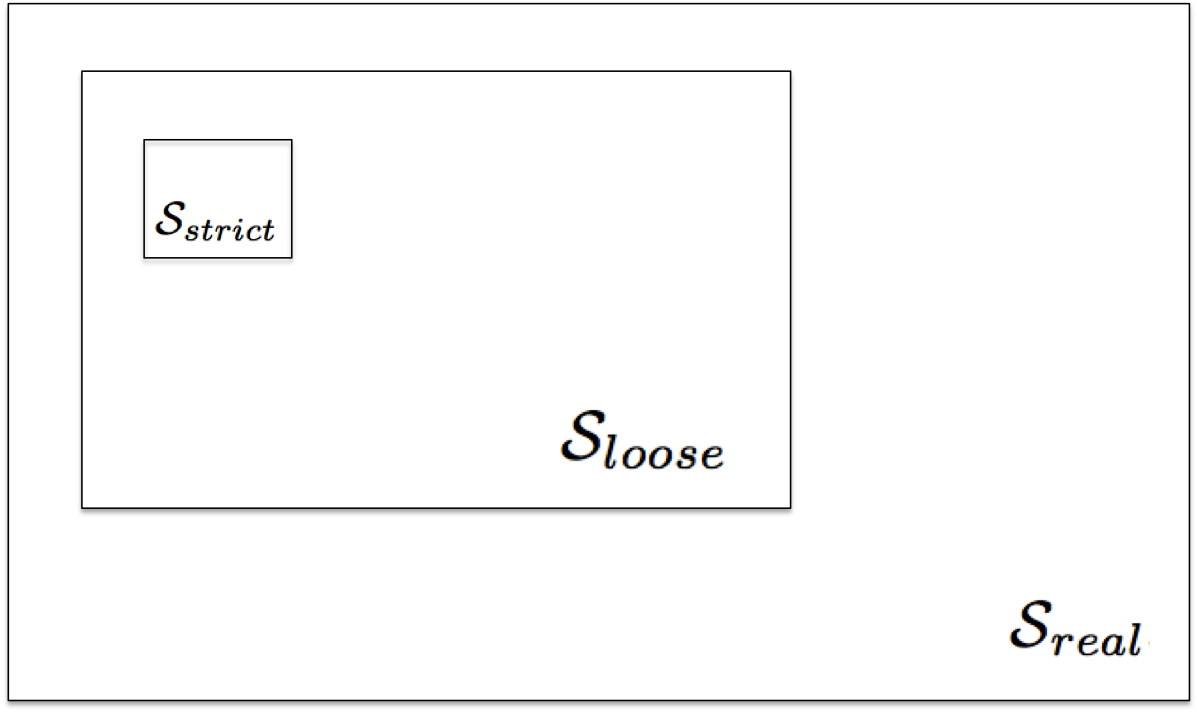
\includegraphics[width=0.7\columnwidth]{Figures/dataset_sizes.png}
	\caption{Representation of our $\mathcal{S}_{strict}$, $\mathcal{S}_{loose}$ and $\mathcal{S}_{real}$ scenarios.}
	\label{fig:scenarios}
\end{figure}

To understand the impacts of temporal consistent learning, we perform a comparative analysis of the three above scenarios under two distinct environments:

\begin{itemize}
	\item \textit{laboratory conditions} where traditional cross-validation methodologies can be applied;
	\item \emph{real-world conditions} where time is relevant and we analyze the behavior of the classifier with temporal-based methodologies.
\end{itemize}

We also provide several improvements to the model.
One of these come under the form of a multi-layer approach, which instead of classifying a sample as malware or goodware, also provides information regarding the type of malware.
Our other improvement regards providing more information about a sample to the model, in order to obtain higher scores.

%%%%%%%%%%%%%%%%%%%%%%%%%%%%%%%%%%%%%%%%%%%%%%%%%%%%%%%%%%%%%%%%%%%%%%%%
\section{Thesis Outline}
\label{section:outline}

Chapter \ref{chapter:related_work} introduces malware by describing some of its history, followed by different techniques to detect malware. We then describe a practical application of a specific analysis technique, from which we obtained our dataset.
We introduce the notion of machine learning and its applications, followed by related work that specifically uses \gls{ml} to detect malware. 

Chapter \ref{chapter:data_collection} describes our initial approach and methodology to help solve the problem of malware detection using \gls{ml}. We detail the data gathering process and how it was analyzed, followed by the labeling process and dataset creation.

Chapter \ref{chapter:static_features} and \ref{chapter:model_improvements} takes the created datasets to build a malware detection model based on both static and dynamic features, as well as how these perform under different validation methodologies.

Chapter \ref{chapter:practical_applications} describes how our model is practically implemented both as an online malware detection service and how it was inserted into a corporate email server to analyze attachments.

Chapter \ref{chapter:conclusions} provides some final remarks on our work and contributions, together with possible ideas that may improve the presented work.
